%\documentclass{standalone}
%\usepackage{tikz}
%\usetikzlibrary{patterns,plotmarks}
%\begin{document}
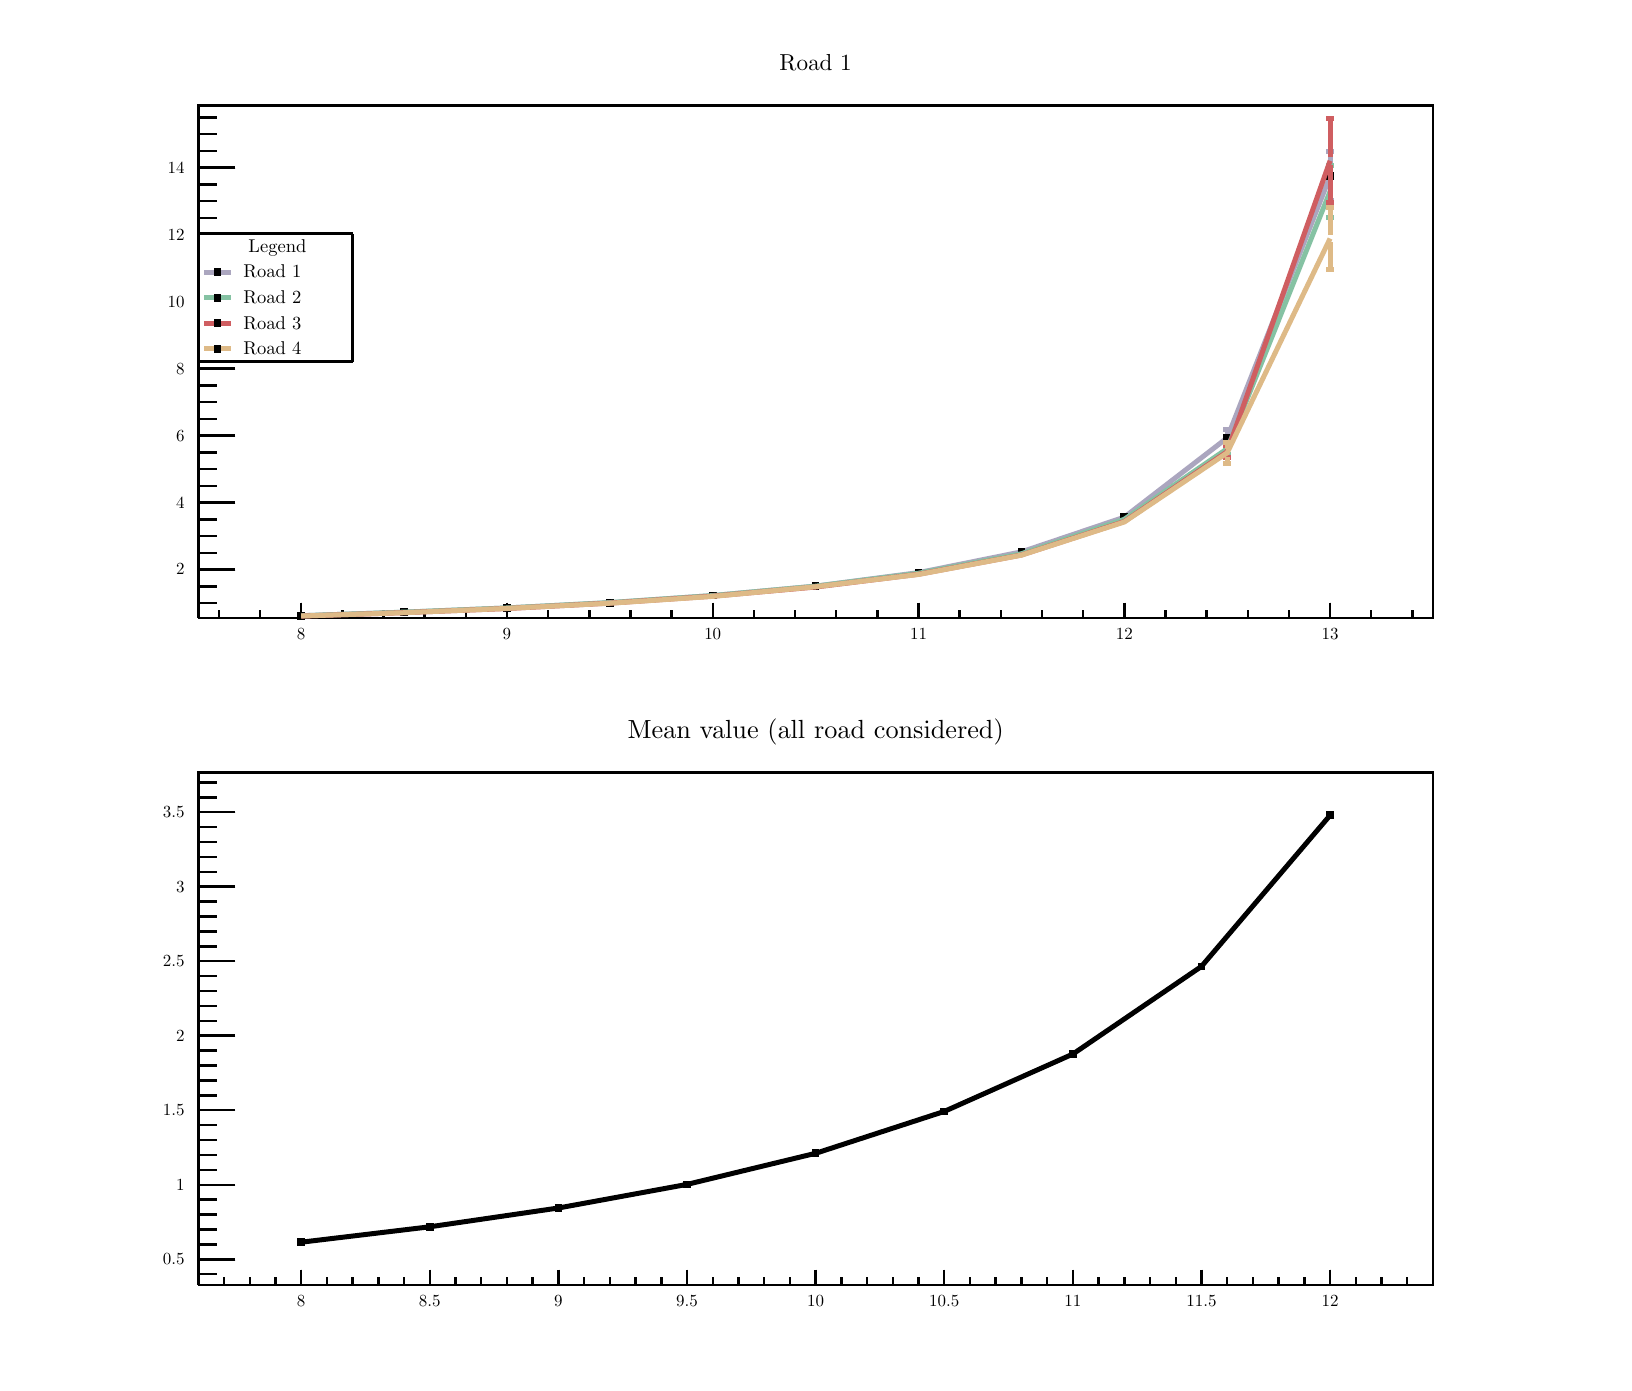
\begin{tikzpicture}
\def\CheckTikzLibraryLoaded#1{ \ifcsname tikz@library@#1@loaded\endcsname \else \PackageWarning{tikz}{usetikzlibrary{#1} is missing in the preamble.} \fi }
\CheckTikzLibraryLoaded{patterns}
\CheckTikzLibraryLoaded{plotmarks}
\pgfdeclareplotmark{cross} {
\pgfpathmoveto{\pgfpoint{-0.3\pgfplotmarksize}{\pgfplotmarksize}}
\pgfpathlineto{\pgfpoint{+0.3\pgfplotmarksize}{\pgfplotmarksize}}
\pgfpathlineto{\pgfpoint{+0.3\pgfplotmarksize}{0.3\pgfplotmarksize}}
\pgfpathlineto{\pgfpoint{+1\pgfplotmarksize}{0.3\pgfplotmarksize}}
\pgfpathlineto{\pgfpoint{+1\pgfplotmarksize}{-0.3\pgfplotmarksize}}
\pgfpathlineto{\pgfpoint{+0.3\pgfplotmarksize}{-0.3\pgfplotmarksize}}
\pgfpathlineto{\pgfpoint{+0.3\pgfplotmarksize}{-1.\pgfplotmarksize}}
\pgfpathlineto{\pgfpoint{-0.3\pgfplotmarksize}{-1.\pgfplotmarksize}}
\pgfpathlineto{\pgfpoint{-0.3\pgfplotmarksize}{-0.3\pgfplotmarksize}}
\pgfpathlineto{\pgfpoint{-1.\pgfplotmarksize}{-0.3\pgfplotmarksize}}
\pgfpathlineto{\pgfpoint{-1.\pgfplotmarksize}{0.3\pgfplotmarksize}}
\pgfpathlineto{\pgfpoint{-0.3\pgfplotmarksize}{0.3\pgfplotmarksize}}
\pgfpathclose
\pgfusepathqstroke
}
\pgfdeclareplotmark{cross*} {
\pgfpathmoveto{\pgfpoint{-0.3\pgfplotmarksize}{\pgfplotmarksize}}
\pgfpathlineto{\pgfpoint{+0.3\pgfplotmarksize}{\pgfplotmarksize}}
\pgfpathlineto{\pgfpoint{+0.3\pgfplotmarksize}{0.3\pgfplotmarksize}}
\pgfpathlineto{\pgfpoint{+1\pgfplotmarksize}{0.3\pgfplotmarksize}}
\pgfpathlineto{\pgfpoint{+1\pgfplotmarksize}{-0.3\pgfplotmarksize}}
\pgfpathlineto{\pgfpoint{+0.3\pgfplotmarksize}{-0.3\pgfplotmarksize}}
\pgfpathlineto{\pgfpoint{+0.3\pgfplotmarksize}{-1.\pgfplotmarksize}}
\pgfpathlineto{\pgfpoint{-0.3\pgfplotmarksize}{-1.\pgfplotmarksize}}
\pgfpathlineto{\pgfpoint{-0.3\pgfplotmarksize}{-0.3\pgfplotmarksize}}
\pgfpathlineto{\pgfpoint{-1.\pgfplotmarksize}{-0.3\pgfplotmarksize}}
\pgfpathlineto{\pgfpoint{-1.\pgfplotmarksize}{0.3\pgfplotmarksize}}
\pgfpathlineto{\pgfpoint{-0.3\pgfplotmarksize}{0.3\pgfplotmarksize}}
\pgfpathclose
\pgfusepathqfillstroke
}
\pgfdeclareplotmark{newstar} {
\pgfpathmoveto{\pgfqpoint{0pt}{\pgfplotmarksize}}
\pgfpathlineto{\pgfqpointpolar{44}{0.5\pgfplotmarksize}}
\pgfpathlineto{\pgfqpointpolar{18}{\pgfplotmarksize}}
\pgfpathlineto{\pgfqpointpolar{-20}{0.5\pgfplotmarksize}}
\pgfpathlineto{\pgfqpointpolar{-54}{\pgfplotmarksize}}
\pgfpathlineto{\pgfqpointpolar{-90}{0.5\pgfplotmarksize}}
\pgfpathlineto{\pgfqpointpolar{234}{\pgfplotmarksize}}
\pgfpathlineto{\pgfqpointpolar{198}{0.5\pgfplotmarksize}}
\pgfpathlineto{\pgfqpointpolar{162}{\pgfplotmarksize}}
\pgfpathlineto{\pgfqpointpolar{134}{0.5\pgfplotmarksize}}
\pgfpathclose
\pgfusepathqstroke
}
\pgfdeclareplotmark{newstar*} {
\pgfpathmoveto{\pgfqpoint{0pt}{\pgfplotmarksize}}
\pgfpathlineto{\pgfqpointpolar{44}{0.5\pgfplotmarksize}}
\pgfpathlineto{\pgfqpointpolar{18}{\pgfplotmarksize}}
\pgfpathlineto{\pgfqpointpolar{-20}{0.5\pgfplotmarksize}}
\pgfpathlineto{\pgfqpointpolar{-54}{\pgfplotmarksize}}
\pgfpathlineto{\pgfqpointpolar{-90}{0.5\pgfplotmarksize}}
\pgfpathlineto{\pgfqpointpolar{234}{\pgfplotmarksize}}
\pgfpathlineto{\pgfqpointpolar{198}{0.5\pgfplotmarksize}}
\pgfpathlineto{\pgfqpointpolar{162}{\pgfplotmarksize}}
\pgfpathlineto{\pgfqpointpolar{134}{0.5\pgfplotmarksize}}
\pgfpathclose
\pgfusepathqfillstroke
}
\definecolor{c}{rgb}{1,1,1};
\draw [color=c, fill=c] (0,0) rectangle (20,16.9424);
\draw [color=c, fill=c] (0.2,8.6406) rectangle (19.8,16.7729);
\draw [color=c, fill=c] (2.16,9.45383) rectangle (17.84,15.9597);
\definecolor{c}{rgb}{0,0,0};
\draw [c,line width=0.9] (2.16,9.45383) -- (2.16,15.9597) -- (17.84,15.9597) -- (17.84,9.45383) -- (2.16,9.45383);
\definecolor{c}{rgb}{1,1,1};
\draw [color=c, fill=c] (2.16,9.45383) rectangle (17.84,15.9597);
\definecolor{c}{rgb}{0,0,0};
\draw [c,line width=0.9] (2.16,9.45383) -- (2.16,15.9597) -- (17.84,15.9597) -- (17.84,9.45383) -- (2.16,9.45383);
\draw [c,line width=0.9] (2.16,9.45383) -- (17.84,9.45383);
\draw [c,line width=0.9] (3.46667,9.64901) -- (3.46667,9.45383);
\draw [c,line width=0.9] (3.98933,9.55142) -- (3.98933,9.45383);
\draw [c,line width=0.9] (4.512,9.55142) -- (4.512,9.45383);
\draw [c,line width=0.9] (5.03467,9.55142) -- (5.03467,9.45383);
\draw [c,line width=0.9] (5.55733,9.55142) -- (5.55733,9.45383);
\draw [c,line width=0.9] (6.08,9.64901) -- (6.08,9.45383);
\draw [c,line width=0.9] (6.60267,9.55142) -- (6.60267,9.45383);
\draw [c,line width=0.9] (7.12533,9.55142) -- (7.12533,9.45383);
\draw [c,line width=0.9] (7.648,9.55142) -- (7.648,9.45383);
\draw [c,line width=0.9] (8.17067,9.55142) -- (8.17067,9.45383);
\draw [c,line width=0.9] (8.69333,9.64901) -- (8.69333,9.45383);
\draw [c,line width=0.9] (9.216,9.55142) -- (9.216,9.45383);
\draw [c,line width=0.9] (9.73867,9.55142) -- (9.73867,9.45383);
\draw [c,line width=0.9] (10.2613,9.55142) -- (10.2613,9.45383);
\draw [c,line width=0.9] (10.784,9.55142) -- (10.784,9.45383);
\draw [c,line width=0.9] (11.3067,9.64901) -- (11.3067,9.45383);
\draw [c,line width=0.9] (11.8293,9.55142) -- (11.8293,9.45383);
\draw [c,line width=0.9] (12.352,9.55142) -- (12.352,9.45383);
\draw [c,line width=0.9] (12.8747,9.55142) -- (12.8747,9.45383);
\draw [c,line width=0.9] (13.3973,9.55142) -- (13.3973,9.45383);
\draw [c,line width=0.9] (13.92,9.64901) -- (13.92,9.45383);
\draw [c,line width=0.9] (14.4427,9.55142) -- (14.4427,9.45383);
\draw [c,line width=0.9] (14.9653,9.55142) -- (14.9653,9.45383);
\draw [c,line width=0.9] (15.488,9.55142) -- (15.488,9.45383);
\draw [c,line width=0.9] (16.0107,9.55142) -- (16.0107,9.45383);
\draw [c,line width=0.9] (16.5333,9.64901) -- (16.5333,9.45383);
\draw [c,line width=0.9] (3.46667,9.64901) -- (3.46667,9.45383);
\draw [c,line width=0.9] (2.944,9.55142) -- (2.944,9.45383);
\draw [c,line width=0.9] (2.42133,9.55142) -- (2.42133,9.45383);
\draw [c,line width=0.9] (16.5333,9.64901) -- (16.5333,9.45383);
\draw [c,line width=0.9] (17.056,9.55142) -- (17.056,9.45383);
\draw [c,line width=0.9] (17.5787,9.55142) -- (17.5787,9.45383);
\draw [anchor=base] (3.46667,9.18547) node[scale=0.613205, color=c, rotate=0]{8};
\draw [anchor=base] (6.08,9.18547) node[scale=0.613205, color=c, rotate=0]{9};
\draw [anchor=base] (8.69333,9.18547) node[scale=0.613205, color=c, rotate=0]{10};
\draw [anchor=base] (11.3067,9.18547) node[scale=0.613205, color=c, rotate=0]{11};
\draw [anchor=base] (13.92,9.18547) node[scale=0.613205, color=c, rotate=0]{12};
\draw [anchor=base] (16.5333,9.18547) node[scale=0.613205, color=c, rotate=0]{13};
\draw [c,line width=0.9] (2.16,9.45383) -- (2.16,15.9597);
\draw [c,line width=0.9] (2.6304,10.0679) -- (2.16,10.0679);
\draw [c,line width=0.9] (2.3952,10.2805) -- (2.16,10.2805);
\draw [c,line width=0.9] (2.3952,10.4931) -- (2.16,10.4931);
\draw [c,line width=0.9] (2.3952,10.7057) -- (2.16,10.7057);
\draw [c,line width=0.9] (2.6304,10.9183) -- (2.16,10.9183);
\draw [c,line width=0.9] (2.3952,11.131) -- (2.16,11.131);
\draw [c,line width=0.9] (2.3952,11.3436) -- (2.16,11.3436);
\draw [c,line width=0.9] (2.3952,11.5562) -- (2.16,11.5562);
\draw [c,line width=0.9] (2.6304,11.7688) -- (2.16,11.7688);
\draw [c,line width=0.9] (2.3952,11.9814) -- (2.16,11.9814);
\draw [c,line width=0.9] (2.3952,12.194) -- (2.16,12.194);
\draw [c,line width=0.9] (2.3952,12.4066) -- (2.16,12.4066);
\draw [c,line width=0.9] (2.6304,12.6192) -- (2.16,12.6192);
\draw [c,line width=0.9] (2.3952,12.8318) -- (2.16,12.8318);
\draw [c,line width=0.9] (2.3952,13.0444) -- (2.16,13.0444);
\draw [c,line width=0.9] (2.3952,13.257) -- (2.16,13.257);
\draw [c,line width=0.9] (2.6304,13.4696) -- (2.16,13.4696);
\draw [c,line width=0.9] (2.3952,13.6822) -- (2.16,13.6822);
\draw [c,line width=0.9] (2.3952,13.8948) -- (2.16,13.8948);
\draw [c,line width=0.9] (2.3952,14.1074) -- (2.16,14.1074);
\draw [c,line width=0.9] (2.6304,14.32) -- (2.16,14.32);
\draw [c,line width=0.9] (2.3952,14.5326) -- (2.16,14.5326);
\draw [c,line width=0.9] (2.3952,14.7452) -- (2.16,14.7452);
\draw [c,line width=0.9] (2.3952,14.9578) -- (2.16,14.9578);
\draw [c,line width=0.9] (2.6304,15.1705) -- (2.16,15.1705);
\draw [c,line width=0.9] (2.6304,10.0679) -- (2.16,10.0679);
\draw [c,line width=0.9] (2.3952,9.85532) -- (2.16,9.85532);
\draw [c,line width=0.9] (2.3952,9.64272) -- (2.16,9.64272);
\draw [c,line width=0.9] (2.6304,15.1705) -- (2.16,15.1705);
\draw [c,line width=0.9] (2.3952,15.3831) -- (2.16,15.3831);
\draw [c,line width=0.9] (2.3952,15.5957) -- (2.16,15.5957);
\draw [c,line width=0.9] (2.3952,15.8083) -- (2.16,15.8083);
\draw [anchor= east] (2.062,10.0679) node[scale=0.613205, color=c, rotate=0]{2};
\draw [anchor= east] (2.062,10.9183) node[scale=0.613205, color=c, rotate=0]{4};
\draw [anchor= east] (2.062,11.7688) node[scale=0.613205, color=c, rotate=0]{6};
\draw [anchor= east] (2.062,12.6192) node[scale=0.613205, color=c, rotate=0]{8};
\draw [anchor= east] (2.062,13.4696) node[scale=0.613205, color=c, rotate=0]{10};
\draw [anchor= east] (2.062,14.32) node[scale=0.613205, color=c, rotate=0]{12};
\draw [anchor= east] (2.062,15.1705) node[scale=0.613205, color=c, rotate=0]{14};
\definecolor{c}{rgb}{0.67,0.65,0.75};
\draw [c,line width=1.8] (3.46667,9.48139) -- (4.77333,9.52529) -- (6.08,9.57989) -- (7.38667,9.64619) -- (8.69333,9.73711) -- (10,9.85697) -- (11.3067,10.0284) -- (12.6133,10.2919) -- (13.92,10.7324) -- (15.2267,11.7396) -- (16.5333,15.0619);
\definecolor{c}{rgb}{0,0,0};
\foreach \P in {(3.46667,9.48139), (4.77333,9.52529), (6.08,9.57989), (7.38667,9.64619), (8.69333,9.73711), (10,9.85697), (11.3067,10.0284), (12.6133,10.2919), (13.92,10.7324), (15.2267,11.7396), (16.5333,15.0619)}{\draw[mark
 options={color=c,fill=c},mark size=1.201201pt, line width=0.000000pt, mark=square*] plot coordinates {\P};}
\definecolor{c}{rgb}{0.67,0.65,0.75};
\draw [c,line width=1.8] (15.2267,11.7897) -- (15.2267,11.8446);
\draw [c,line width=1.8] (15.1765,11.8446) -- (15.2768,11.8446);
\draw [c,line width=1.8] (15.2267,11.6894) -- (15.2267,11.6345);
\draw [c,line width=1.8] (15.1765,11.6345) -- (15.2768,11.6345);
\draw [c,line width=1.8] (16.5333,15.112) -- (16.5333,15.3706);
\draw [c,line width=1.8] (16.4832,15.3706) -- (16.5835,15.3706);
\draw [c,line width=1.8] (16.5333,15.0118) -- (16.5333,14.7531);
\draw [c,line width=1.8] (16.4832,14.7531) -- (16.5835,14.7531);
\definecolor{c}{rgb}{0.52,0.76,0.64};
\draw [c,line width=1.8] (15.2267,11.6519) -- (15.2267,11.6751);
\draw [c,line width=1.8] (15.1765,11.6751) -- (15.2768,11.6751);
\draw [c,line width=1.8] (15.2267,11.5516) -- (15.2267,11.5284);
\draw [c,line width=1.8] (15.1765,11.5284) -- (15.2768,11.5284);
\draw [c,line width=1.8] (16.5333,14.9198) -- (16.5333,15.1966);
\draw [c,line width=1.8] (16.4832,15.1966) -- (16.5835,15.1966);
\draw [c,line width=1.8] (16.5333,14.8196) -- (16.5333,14.5428);
\draw [c,line width=1.8] (16.4832,14.5428) -- (16.5835,14.5428);
\draw [c,line width=1.8] (3.46667,9.48062) -- (4.77333,9.5266) -- (6.08,9.57967) -- (7.38667,9.64808) -- (8.69333,9.73695) -- (10,9.85609) -- (11.3067,10.021) -- (12.6133,10.2685) -- (13.92,10.7058) -- (15.2267,11.6018) -- (16.5333,14.8697);
\definecolor{c}{rgb}{0.81,0.37,0.38};
\draw [c,line width=1.8] (15.2267,11.6148) -- (15.2267,11.6411);
\draw [c,line width=1.8] (15.1765,11.6411) -- (15.2768,11.6411);
\draw [c,line width=1.8] (15.2267,11.5146) -- (15.2267,11.4883);
\draw [c,line width=1.8] (15.1765,11.4883) -- (15.2768,11.4883);
\draw [c,line width=1.8] (16.5333,15.3091) -- (16.5333,15.7928);
\draw [c,line width=1.8] (16.4832,15.7928) -- (16.5835,15.7928);
\draw [c,line width=1.8] (16.5333,15.2088) -- (16.5333,14.7251);
\draw [c,line width=1.8] (16.4832,14.7251) -- (16.5835,14.7251);
\draw [c,line width=1.8] (3.46667,9.47637) -- (4.77333,9.52014) -- (6.08,9.5726) -- (7.38667,9.64122) -- (8.69333,9.72935) -- (10,9.84573) -- (11.3067,10.0079) -- (12.6133,10.2521) -- (13.92,10.6776) -- (15.2267,11.5647) -- (16.5333,15.259);
\definecolor{c}{rgb}{0.87,0.73,0.53};
\draw [c,line width=1.8] (15.2267,11.6002) -- (15.2267,11.6807);
\draw [c,line width=1.8] (15.1765,11.6807) -- (15.2768,11.6807);
\draw [c,line width=1.8] (15.2267,11.4999) -- (15.2267,11.4194);
\draw [c,line width=1.8] (15.1765,11.4194) -- (15.2768,11.4194);
\draw [c,line width=1.8] (16.5333,14.3214) -- (16.5333,14.6651);
\draw [c,line width=1.8] (16.4832,14.6651) -- (16.5835,14.6651);
\draw [c,line width=1.8] (16.5333,14.2212) -- (16.5333,13.8775);
\draw [c,line width=1.8] (16.4832,13.8775) -- (16.5835,13.8775);
\draw [c,line width=1.8] (3.46667,9.47709) -- (4.77333,9.51937) -- (6.08,9.57374) -- (7.38667,9.63965) -- (8.69333,9.72662) -- (10,9.84892) -- (11.3067,10.0052) -- (12.6133,10.2502) -- (13.92,10.6714) -- (15.2267,11.5501) -- (16.5333,14.2713);
\definecolor{c}{rgb}{1,1,1};
\draw [color=c, fill=c] (2.16,12.7068) rectangle (4.12,14.3332);
\definecolor{c}{rgb}{0,0,0};
\draw [c,line width=0.9] (2.16,12.7068) -- (4.12,12.7068);
\draw [c,line width=0.9] (4.12,12.7068) -- (4.12,14.3332);
\draw [c,line width=0.9] (4.12,14.3332) -- (2.16,14.3332);
\draw [c,line width=0.9] (2.16,14.3332) -- (2.16,12.7068);
\draw [anchor=base] (3.1645,14.0974) node[scale=0.66895, color=c, rotate=0]{Legend};
\draw [anchor=base west] (2.65,13.7721) node[scale=0.66895, color=c, rotate=0]{Road 1};
\definecolor{c}{rgb}{1,1,1};
\draw [c, fill=c] (2.2335,13.7314) -- (2.5765,13.7314) -- (2.5765,13.9591) -- (2.2335,13.9591);
\definecolor{c}{rgb}{0.67,0.65,0.75};
\draw [c,line width=1.8] (2.2335,13.8453) -- (2.5765,13.8453);
\definecolor{c}{rgb}{0,0,0};
\foreach \P in {(2.405,13.8453)}{\draw[mark options={color=c,fill=c},mark size=1.201201pt, line width=0.000000pt, mark=square*] plot coordinates {\P};}
\draw [anchor=base west] (2.65,13.4468) node[scale=0.66895, color=c, rotate=0]{Road 2};
\definecolor{c}{rgb}{1,1,1};
\draw [c, fill=c] (2.2335,13.4061) -- (2.5765,13.4061) -- (2.5765,13.6339) -- (2.2335,13.6339);
\definecolor{c}{rgb}{0.52,0.76,0.64};
\draw [c,line width=1.8] (2.2335,13.52) -- (2.5765,13.52);
\definecolor{c}{rgb}{0,0,0};
\foreach \P in {(2.405,13.52)}{\draw[mark options={color=c,fill=c},mark size=1.201201pt, line width=0.000000pt, mark=square*] plot coordinates {\P};}
\draw [anchor=base west] (2.65,13.1215) node[scale=0.66895, color=c, rotate=0]{Road 3};
\definecolor{c}{rgb}{1,1,1};
\draw [c, fill=c] (2.2335,13.0809) -- (2.5765,13.0809) -- (2.5765,13.3086) -- (2.2335,13.3086);
\definecolor{c}{rgb}{0.81,0.37,0.38};
\draw [c,line width=1.8] (2.2335,13.1947) -- (2.5765,13.1947);
\definecolor{c}{rgb}{0,0,0};
\foreach \P in {(2.405,13.1947)}{\draw[mark options={color=c,fill=c},mark size=1.201201pt, line width=0.000000pt, mark=square*] plot coordinates {\P};}
\draw [anchor=base west] (2.65,12.7962) node[scale=0.66895, color=c, rotate=0]{Road 4};
\definecolor{c}{rgb}{1,1,1};
\draw [c, fill=c] (2.2335,12.7556) -- (2.5765,12.7556) -- (2.5765,12.9833) -- (2.2335,12.9833);
\definecolor{c}{rgb}{0.87,0.73,0.53};
\draw [c,line width=1.8] (2.2335,12.8694) -- (2.5765,12.8694);
\definecolor{c}{rgb}{0,0,0};
\foreach \P in {(2.405,12.8694)}{\draw[mark options={color=c,fill=c},mark size=1.201201pt, line width=0.000000pt, mark=square*] plot coordinates {\P};}
\draw (10,16.5086) node[scale=0.836188, color=c, rotate=0]{Road 1};
\definecolor{c}{rgb}{1,1,1};
\draw [color=c, fill=c] (0.2,0.169424) rectangle (19.8,8.30175);
\draw [color=c, fill=c] (2.16,0.982657) rectangle (17.84,7.48852);
\definecolor{c}{rgb}{0,0,0};
\draw [c,line width=0.9] (2.16,0.982657) -- (2.16,7.48852) -- (17.84,7.48852) -- (17.84,0.982657) -- (2.16,0.982657);
\definecolor{c}{rgb}{1,1,1};
\draw [color=c, fill=c] (2.16,0.982657) rectangle (17.84,7.48852);
\definecolor{c}{rgb}{0,0,0};
\draw [c,line width=0.9] (2.16,0.982657) -- (2.16,7.48852) -- (17.84,7.48852) -- (17.84,0.982657) -- (2.16,0.982657);
\draw [c,line width=0.9] (2.16,0.982657) -- (17.84,0.982657);
\draw [c,line width=0.9] (3.46667,1.17783) -- (3.46667,0.982657);
\draw [c,line width=0.9] (3.79333,1.08024) -- (3.79333,0.982657);
\draw [c,line width=0.9] (4.12,1.08024) -- (4.12,0.982657);
\draw [c,line width=0.9] (4.44667,1.08024) -- (4.44667,0.982657);
\draw [c,line width=0.9] (4.77333,1.08024) -- (4.77333,0.982657);
\draw [c,line width=0.9] (5.1,1.17783) -- (5.1,0.982657);
\draw [c,line width=0.9] (5.42667,1.08024) -- (5.42667,0.982657);
\draw [c,line width=0.9] (5.75333,1.08024) -- (5.75333,0.982657);
\draw [c,line width=0.9] (6.08,1.08024) -- (6.08,0.982657);
\draw [c,line width=0.9] (6.40667,1.08024) -- (6.40667,0.982657);
\draw [c,line width=0.9] (6.73333,1.17783) -- (6.73333,0.982657);
\draw [c,line width=0.9] (7.06,1.08024) -- (7.06,0.982657);
\draw [c,line width=0.9] (7.38667,1.08024) -- (7.38667,0.982657);
\draw [c,line width=0.9] (7.71333,1.08024) -- (7.71333,0.982657);
\draw [c,line width=0.9] (8.04,1.08024) -- (8.04,0.982657);
\draw [c,line width=0.9] (8.36667,1.17783) -- (8.36667,0.982657);
\draw [c,line width=0.9] (8.69333,1.08024) -- (8.69333,0.982657);
\draw [c,line width=0.9] (9.02,1.08024) -- (9.02,0.982657);
\draw [c,line width=0.9] (9.34667,1.08024) -- (9.34667,0.982657);
\draw [c,line width=0.9] (9.67333,1.08024) -- (9.67333,0.982657);
\draw [c,line width=0.9] (10,1.17783) -- (10,0.982657);
\draw [c,line width=0.9] (10.3267,1.08024) -- (10.3267,0.982657);
\draw [c,line width=0.9] (10.6533,1.08024) -- (10.6533,0.982657);
\draw [c,line width=0.9] (10.98,1.08024) -- (10.98,0.982657);
\draw [c,line width=0.9] (11.3067,1.08024) -- (11.3067,0.982657);
\draw [c,line width=0.9] (11.6333,1.17783) -- (11.6333,0.982657);
\draw [c,line width=0.9] (11.96,1.08024) -- (11.96,0.982657);
\draw [c,line width=0.9] (12.2867,1.08024) -- (12.2867,0.982657);
\draw [c,line width=0.9] (12.6133,1.08024) -- (12.6133,0.982657);
\draw [c,line width=0.9] (12.94,1.08024) -- (12.94,0.982657);
\draw [c,line width=0.9] (13.2667,1.17783) -- (13.2667,0.982657);
\draw [c,line width=0.9] (13.5933,1.08024) -- (13.5933,0.982657);
\draw [c,line width=0.9] (13.92,1.08024) -- (13.92,0.982657);
\draw [c,line width=0.9] (14.2467,1.08024) -- (14.2467,0.982657);
\draw [c,line width=0.9] (14.5733,1.08024) -- (14.5733,0.982657);
\draw [c,line width=0.9] (14.9,1.17783) -- (14.9,0.982657);
\draw [c,line width=0.9] (15.2267,1.08024) -- (15.2267,0.982657);
\draw [c,line width=0.9] (15.5533,1.08024) -- (15.5533,0.982657);
\draw [c,line width=0.9] (15.88,1.08024) -- (15.88,0.982657);
\draw [c,line width=0.9] (16.2067,1.08024) -- (16.2067,0.982657);
\draw [c,line width=0.9] (16.5333,1.17783) -- (16.5333,0.982657);
\draw [c,line width=0.9] (3.46667,1.17783) -- (3.46667,0.982657);
\draw [c,line width=0.9] (3.14,1.08024) -- (3.14,0.982657);
\draw [c,line width=0.9] (2.81333,1.08024) -- (2.81333,0.982657);
\draw [c,line width=0.9] (2.48667,1.08024) -- (2.48667,0.982657);
\draw [c,line width=0.9] (2.16,1.08024) -- (2.16,0.982657);
\draw [c,line width=0.9] (16.5333,1.17783) -- (16.5333,0.982657);
\draw [c,line width=0.9] (16.86,1.08024) -- (16.86,0.982657);
\draw [c,line width=0.9] (17.1867,1.08024) -- (17.1867,0.982657);
\draw [c,line width=0.9] (17.5133,1.08024) -- (17.5133,0.982657);
\draw [c,line width=0.9] (17.84,1.08024) -- (17.84,0.982657);
\draw [anchor=base] (3.46667,0.71429) node[scale=0.613205, color=c, rotate=0]{8};
\draw [anchor=base] (5.1,0.71429) node[scale=0.613205, color=c, rotate=0]{8.5};
\draw [anchor=base] (6.73333,0.71429) node[scale=0.613205, color=c, rotate=0]{9};
\draw [anchor=base] (8.36667,0.71429) node[scale=0.613205, color=c, rotate=0]{9.5};
\draw [anchor=base] (10,0.71429) node[scale=0.613205, color=c, rotate=0]{10};
\draw [anchor=base] (11.6333,0.71429) node[scale=0.613205, color=c, rotate=0]{10.5};
\draw [anchor=base] (13.2667,0.71429) node[scale=0.613205, color=c, rotate=0]{11};
\draw [anchor=base] (14.9,0.71429) node[scale=0.613205, color=c, rotate=0]{11.5};
\draw [anchor=base] (16.5333,0.71429) node[scale=0.613205, color=c, rotate=0]{12};
\draw [c,line width=0.9] (2.16,0.982657) -- (2.16,7.48852);
\draw [c,line width=0.9] (2.6304,1.30779) -- (2.16,1.30779);
\draw [c,line width=0.9] (2.3952,1.49707) -- (2.16,1.49707);
\draw [c,line width=0.9] (2.3952,1.68635) -- (2.16,1.68635);
\draw [c,line width=0.9] (2.3952,1.87563) -- (2.16,1.87563);
\draw [c,line width=0.9] (2.3952,2.06492) -- (2.16,2.06492);
\draw [c,line width=0.9] (2.6304,2.2542) -- (2.16,2.2542);
\draw [c,line width=0.9] (2.3952,2.44348) -- (2.16,2.44348);
\draw [c,line width=0.9] (2.3952,2.63277) -- (2.16,2.63277);
\draw [c,line width=0.9] (2.3952,2.82205) -- (2.16,2.82205);
\draw [c,line width=0.9] (2.3952,3.01133) -- (2.16,3.01133);
\draw [c,line width=0.9] (2.6304,3.20062) -- (2.16,3.20062);
\draw [c,line width=0.9] (2.3952,3.3899) -- (2.16,3.3899);
\draw [c,line width=0.9] (2.3952,3.57918) -- (2.16,3.57918);
\draw [c,line width=0.9] (2.3952,3.76847) -- (2.16,3.76847);
\draw [c,line width=0.9] (2.3952,3.95775) -- (2.16,3.95775);
\draw [c,line width=0.9] (2.6304,4.14703) -- (2.16,4.14703);
\draw [c,line width=0.9] (2.3952,4.33632) -- (2.16,4.33632);
\draw [c,line width=0.9] (2.3952,4.5256) -- (2.16,4.5256);
\draw [c,line width=0.9] (2.3952,4.71488) -- (2.16,4.71488);
\draw [c,line width=0.9] (2.3952,4.90417) -- (2.16,4.90417);
\draw [c,line width=0.9] (2.6304,5.09345) -- (2.16,5.09345);
\draw [c,line width=0.9] (2.3952,5.28273) -- (2.16,5.28273);
\draw [c,line width=0.9] (2.3952,5.47202) -- (2.16,5.47202);
\draw [c,line width=0.9] (2.3952,5.6613) -- (2.16,5.6613);
\draw [c,line width=0.9] (2.3952,5.85058) -- (2.16,5.85058);
\draw [c,line width=0.9] (2.6304,6.03987) -- (2.16,6.03987);
\draw [c,line width=0.9] (2.3952,6.22915) -- (2.16,6.22915);
\draw [c,line width=0.9] (2.3952,6.41843) -- (2.16,6.41843);
\draw [c,line width=0.9] (2.3952,6.60772) -- (2.16,6.60772);
\draw [c,line width=0.9] (2.3952,6.797) -- (2.16,6.797);
\draw [c,line width=0.9] (2.6304,6.98628) -- (2.16,6.98628);
\draw [c,line width=0.9] (2.6304,1.30779) -- (2.16,1.30779);
\draw [c,line width=0.9] (2.3952,1.1185) -- (2.16,1.1185);
\draw [c,line width=0.9] (2.6304,6.98628) -- (2.16,6.98628);
\draw [c,line width=0.9] (2.3952,7.17557) -- (2.16,7.17557);
\draw [c,line width=0.9] (2.3952,7.36485) -- (2.16,7.36485);
\draw [anchor= east] (2.062,1.30779) node[scale=0.613205, color=c, rotate=0]{0.5};
\draw [anchor= east] (2.062,2.2542) node[scale=0.613205, color=c, rotate=0]{1};
\draw [anchor= east] (2.062,3.20062) node[scale=0.613205, color=c, rotate=0]{1.5};
\draw [anchor= east] (2.062,4.14703) node[scale=0.613205, color=c, rotate=0]{2};
\draw [anchor= east] (2.062,5.09345) node[scale=0.613205, color=c, rotate=0]{2.5};
\draw [anchor= east] (2.062,6.03987) node[scale=0.613205, color=c, rotate=0]{3};
\draw [anchor= east] (2.062,6.98628) node[scale=0.613205, color=c, rotate=0]{3.5};
\draw [c,line width=1.8] (3.46667,1.52481) -- (5.1,1.7206) -- (6.73333,1.95933) -- (8.36667,2.25896) -- (10,2.65391) -- (11.6333,3.1855) -- (13.2667,3.91421) -- (14.9,5.02739) -- (16.5333,6.94637);
\foreach \P in {(3.46667,1.52481), (5.1,1.7206), (6.73333,1.95933), (8.36667,2.25896), (10,2.65391), (11.6333,3.1855), (13.2667,3.91421), (14.9,5.02739), (16.5333,6.94637)}{\draw[mark options={color=c,fill=c},mark size=1.201201pt, line
 width=0.000000pt, mark=square*] plot coordinates {\P};}
\draw (10,8.00545) node[scale=0.94768, color=c, rotate=0]{Mean value (all road considered)};
\end{tikzpicture}
%\end{document}
